% linux-mcp invocation lifecycle (sequence diagram).
% Standalone; compile with: pdflatex linux-mcp-workload.tex
\documentclass[tikz,border=4pt]{standalone}
\usepackage{tikz}
\usepackage{inconsolata}
\usetikzlibrary{positioning,calc,arrows.meta,fit,backgrounds}

\definecolor{edgeDark}{RGB}{70,70,70}
\definecolor{userBand}{RGB}{247,249,252}
\definecolor{kernBand}{RGB}{240,240,240}
\definecolor{phase}{RGB}{210,150,30}
\definecolor{altEdge}{RGB}{180,70,70}

\begin{document}
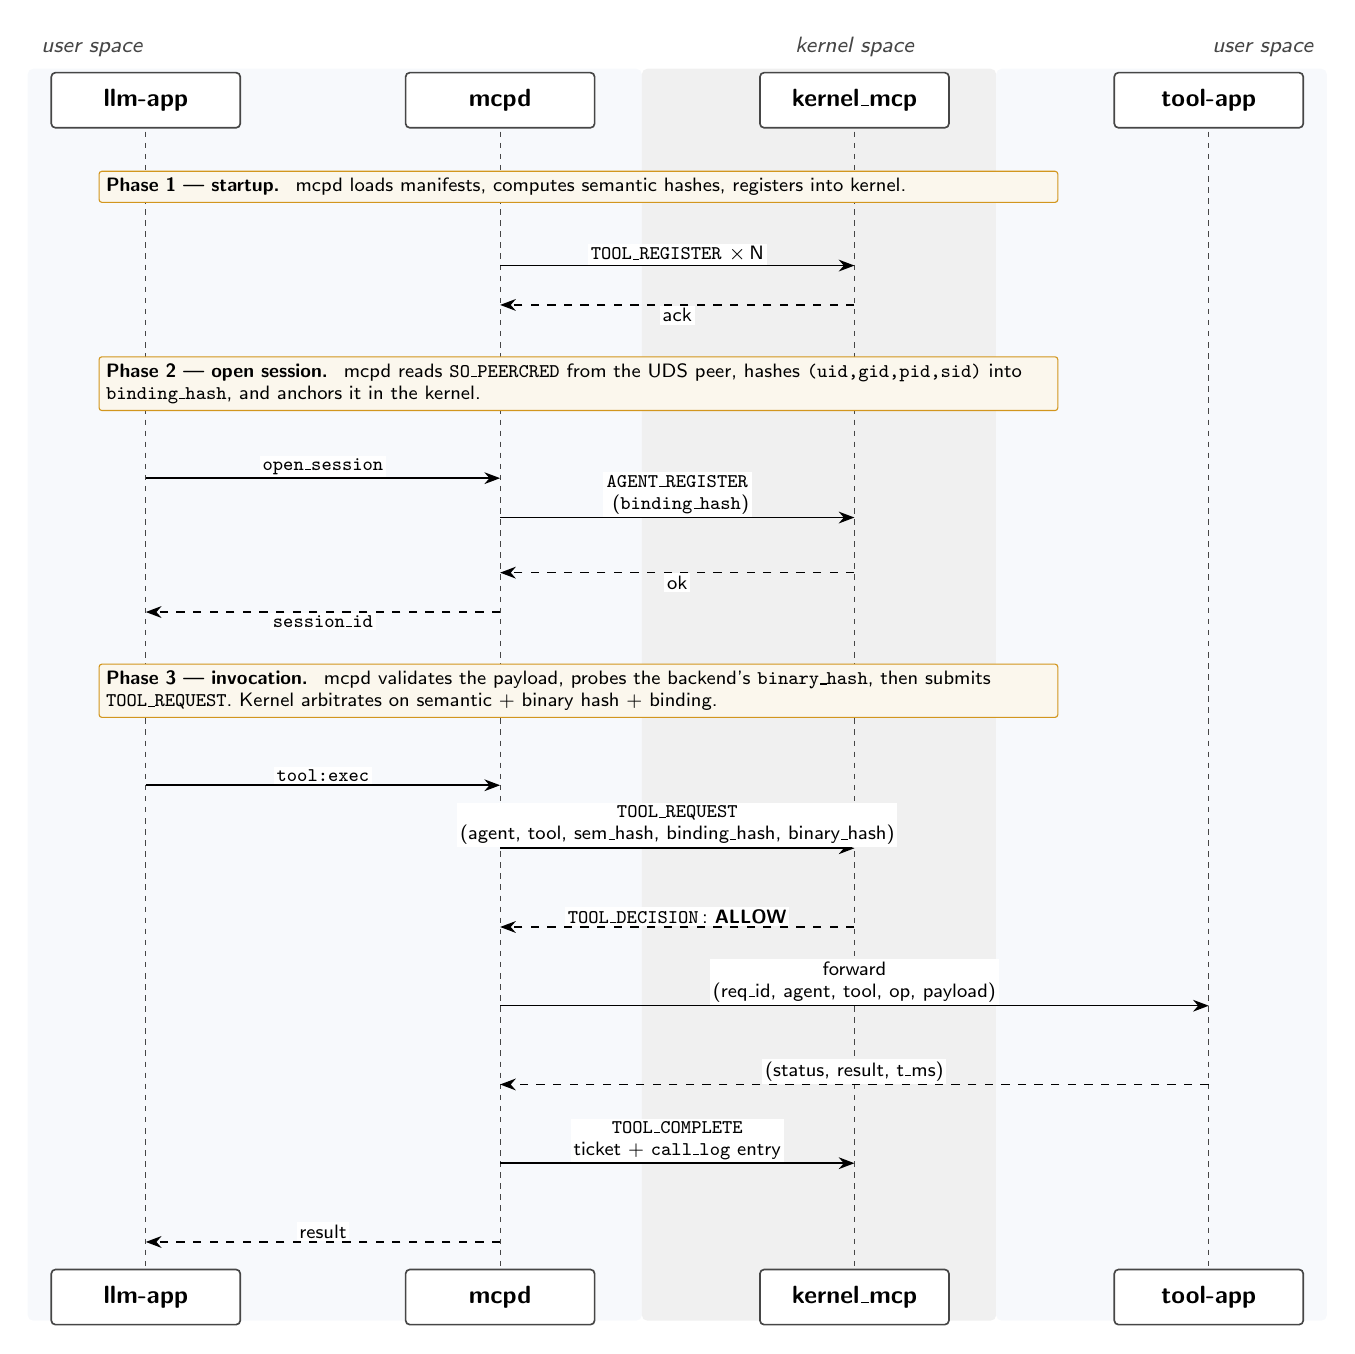
\begin{tikzpicture}[
  font=\small\sffamily,
  head/.style={draw=edgeDark,fill=white,rounded corners=1.5pt,
               minimum width=24mm,minimum height=7mm,line width=0.6pt,
               font=\small\sffamily\bfseries},
  life/.style={line width=0.35pt,dash pattern=on 2pt off 2pt,draw=edgeDark},
  msg/.style={-{Stealth[length=2mm]},line width=0.55pt},
  ret/.style={-{Stealth[length=2mm]},line width=0.55pt,dashed},
  lbl/.style={font=\scriptsize\sffamily,fill=white,inner sep=1pt,align=center},
  phasenote/.style={draw=phase,fill=phase!8,rounded corners=1pt,
                    font=\scriptsize\sffamily,align=left,inner sep=2.5pt,
                    text width=120mm},
  altnote/.style={draw=altEdge,fill=altEdge!5,rounded corners=1pt,
                  font=\scriptsize\sffamily,align=left,inner sep=3pt,
                  text width=128mm}
]

% ---- columns (narrower, closer together) ----
\def\xL{0}     % llm-app
\def\xM{45}    % mcpd
\def\xK{90}    % kernel_mcp
\def\xT{135}   % tool-app

\def\yEnd{-152mm}

% ---- lifeline heads (top) ----
\node[head] (hL) at (\xL mm,0)  {llm-app};
\node[head] (hM) at (\xM mm,0)  {mcpd};
\node[head] (hK) at (\xK mm,0)  {kernel\_mcp};
\node[head] (hT) at (\xT mm,0)  {tool-app};

% ---- lifelines ----
\foreach \X in {\xL,\xM,\xK,\xT}{
  \draw[life] (\X mm,-4mm) -- (\X mm,\yEnd+2mm);
}

% ========================================================
%  Phase 1 — startup
% ========================================================
\node[phasenote,anchor=west] at (-6mm,-11mm)
  {\textbf{\textsf{Phase 1 — startup.}}\;
   mcpd loads manifests, computes semantic hashes, registers into kernel.};

\draw[msg] (\xM mm,-21mm) -- node[lbl,above]{\texttt{TOOL\_REGISTER} $\times$\,N} (\xK mm,-21mm);
\draw[ret] (\xK mm,-26mm) -- node[lbl,below]{ack} (\xM mm,-26mm);

% ========================================================
%  Phase 2 — open session
% ========================================================
\node[phasenote,anchor=west] at (-6mm,-36mm)
  {\textbf{\textsf{Phase 2 — open session.}}\;
   mcpd reads \texttt{SO\_PEERCRED} from the UDS peer, hashes \texttt{(uid,gid,pid,sid)} into \texttt{binding\_hash}, and anchors it in the kernel.};

\draw[msg] (\xL mm,-48mm) -- node[lbl,above]{\texttt{open\_session}} (\xM mm,-48mm);
\draw[msg] (\xM mm,-53mm) -- node[lbl,above,align=center]
  {\texttt{AGENT\_REGISTER}\\\,\,(\texttt{binding\_hash})} (\xK mm,-53mm);
\draw[ret] (\xK mm,-60mm) -- node[lbl,below]{ok} (\xM mm,-60mm);
\draw[ret] (\xM mm,-65mm) -- node[lbl,below]{\texttt{session\_id}} (\xL mm,-65mm);

% ========================================================
%  Phase 3 — invocation
% ========================================================
\node[phasenote,anchor=west] at (-6mm,-75mm)
  {\textbf{\textsf{Phase 3 — invocation.}}\;
   mcpd validates the payload, probes the backend's \texttt{binary\_hash}, then submits \texttt{TOOL\_REQUEST}. Kernel arbitrates on semantic + binary hash + binding.};

\draw[msg] (\xL mm,-87mm) -- node[lbl,above]{\texttt{tool:exec}} (\xM mm,-87mm);

\draw[msg] (\xM mm,-95mm) -- node[lbl,above,align=center]
  {\texttt{TOOL\_REQUEST}\\\scriptsize (agent, tool, sem\_hash, binding\_hash, binary\_hash)}
  (\xK mm,-95mm);

\draw[ret] (\xK mm,-105mm) -- node[lbl,above,align=center]
  {\texttt{TOOL\_DECISION}\,: \textbf{ALLOW}} (\xM mm,-105mm);

\draw[msg] (\xM mm,-115mm) -- node[lbl,above,align=center]
  {forward\\\scriptsize (req\_id, agent, tool, op, payload)} (\xT mm,-115mm);
\draw[ret] (\xT mm,-125mm) -- node[lbl,above]{(status, result, t\_ms)} (\xM mm,-125mm);

\draw[msg] (\xM mm,-135mm) -- node[lbl,above,align=center]
  {\texttt{TOOL\_COMPLETE}\\\scriptsize ticket + \texttt{call\_log} entry} (\xK mm,-135mm);
\draw[ret] (\xM mm,-145mm) -- node[lbl,above]{result} (\xL mm,-145mm);

% ========================================================
%  Alt decisions (compact note, two columns of text)
% ========================================================
% (alt-outcomes note removed by request; DENY/DEFER semantics are in the caption.)

% ---- bands (user / kernel columns) ----
\begin{pgfonlayer}{background}
  \fill[userBand,rounded corners=2pt]
    (\xL mm-15mm, 4mm) rectangle (\xM mm+18mm, \yEnd-3mm);
  \fill[kernBand,rounded corners=2pt]
    (\xM mm+18mm, 4mm) rectangle (\xK mm+18mm, \yEnd-3mm);
  \fill[userBand,rounded corners=2pt]
    (\xK mm+18mm, 4mm) rectangle (\xT mm+15mm, \yEnd-3mm);
\end{pgfonlayer}
\node[font=\footnotesize\sffamily\itshape,text=edgeDark,anchor=south west]
  at (\xL mm-14.5mm, 4.3mm) {user space};
\node[font=\footnotesize\sffamily\itshape,text=edgeDark,anchor=south]
  at (\xK mm, 4.3mm) {kernel space};
\node[font=\footnotesize\sffamily\itshape,text=edgeDark,anchor=south east]
  at (\xT mm+14.5mm, 4.3mm) {user space};

% ---- lifeline heads (bottom, just above alt note) ----
\node[head] at (\xL mm,\yEnd)  {llm-app};
\node[head] at (\xM mm,\yEnd)  {mcpd};
\node[head] at (\xK mm,\yEnd)  {kernel\_mcp};
\node[head] at (\xT mm,\yEnd)  {tool-app};

\end{tikzpicture}
\end{document}
